\section{Methods}

\subsection{MABE: Modular Agent-Based Evolver}

For the experiments in this work we used MABE, the Modular Agent Based Evolver framework \citep{bohm_mabe_2017}. 
We have configured MABE so that agents have a \textbf{genome} (a collection of heritable and mutable data) and a \textbf{brain} (a computational structure that receives input and generates output) specified by the genome. 
MABE manages the evolution of populations of agents by repeatedly evaluating agents in \textbf{worlds} (a fitness-bearing task) and using the results to select parents whose mutated offspring make up future generations. 
The advantage of the MABE framework is that the brains and worlds are completely modularized and therefore can be easily exchanged without altering other system properties, allowing for fast, direct comparisons. 
This ``plug-and-play" feature makes MABE well suited to not only our current cross-brain and cross-world examination, but also to the proposed future extensions of this work.

\subsection{Brains: RNNs and Markov Brains}

In MABE, a brain is a process that converts a list of values \textit{$T_0$} to a new list of values \textit{$T_1$} (Fig~\ref{fig:brains}A). 
We define the $T_0$ values as inputs (i.e. sensor readings or the state of the task) combined with the brain's memory and we define the $T_1$ values as outputs (i.e. values that determine behavior) combined with new memory values (which will be provided to the brain on the next update). 
Each time we want the brain to act (i.e. ask the brain ``what will you do now?") we set the $T_0$ values, allow the brain to run its internal process, and read the resulting $T_1$ values. 

For this work, we compare two well-studied computational structures: RNNs and Markov Brains. 
These structures can be implemented in a number of ways; we describe here our particular implementations. 
It is important to note that these particular implementations are designed not for speed of computation, but for ease of structural analysis.

In all of the experiments described in this work, both the RNNs and Markov Brains have eight memory values.

\begin{figure*}
    \centering
    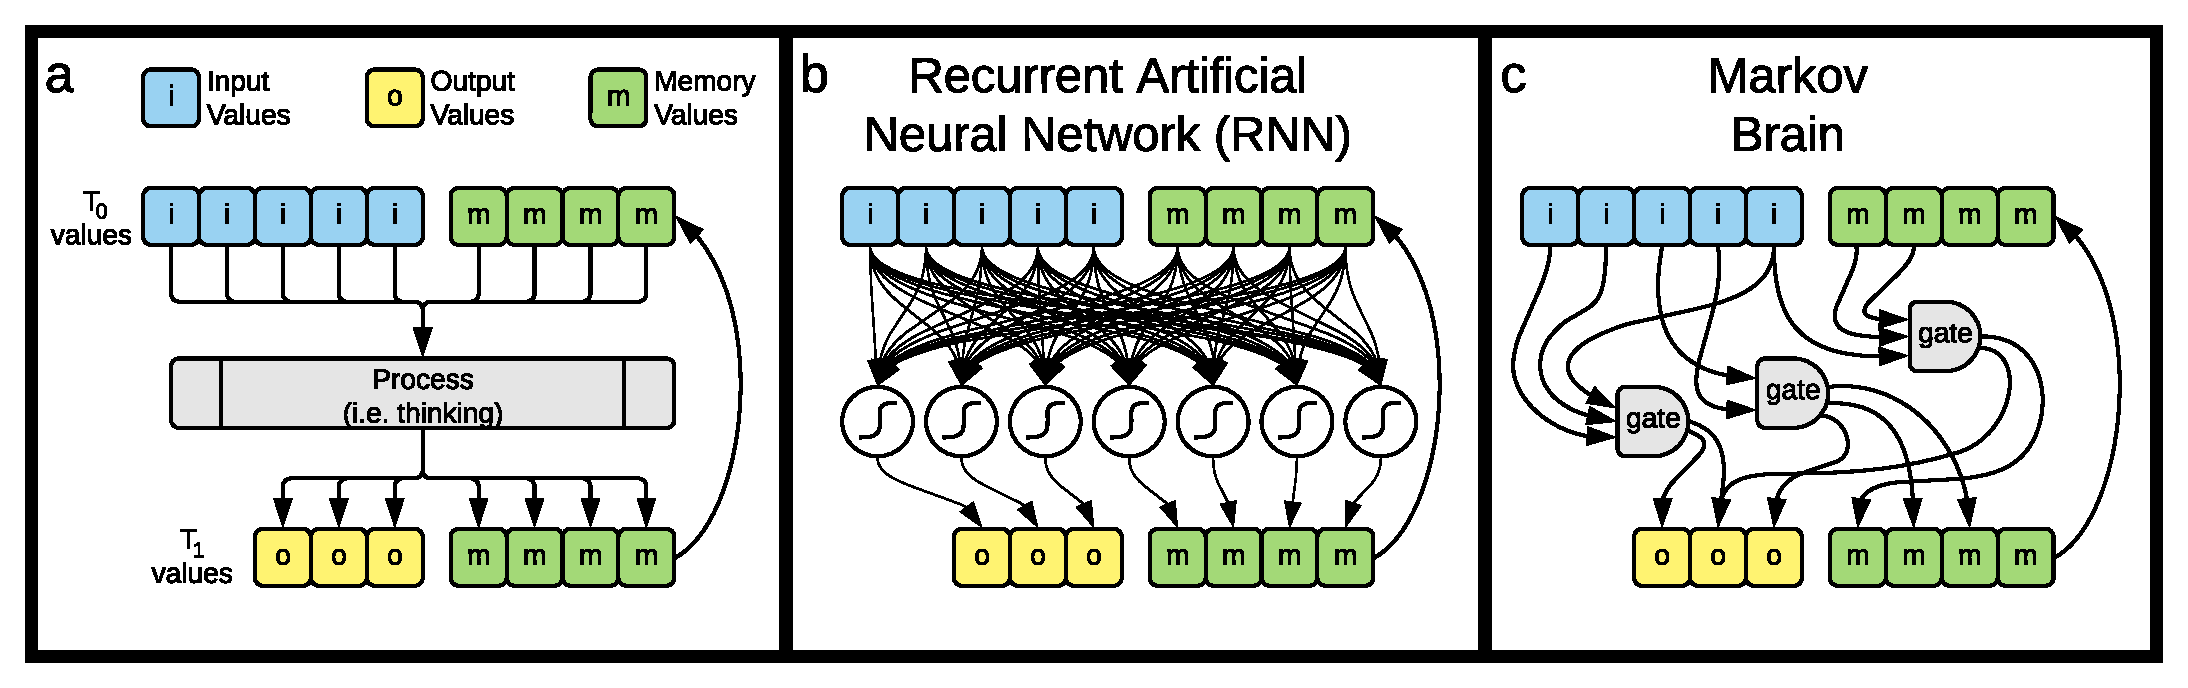
\includegraphics[width=\textwidth]{chapters/2-comp-hybrid/figs/ALIFE_2021_SI_Brains.pdf}
    \caption{Schematics showing structures of A) a generic brain, B) an Recurrent Artificial Neural Network (RNN) and C) a Markov Brain.}
    \label{fig:brains}
\end{figure*}

\subsubsection {Recurrent Artificial Neural Networks:}
RNNs are a well-studied digital neural architecture; see \cite{yu_review_2019} for a review focused on RNNs and learning. 
Typically, RNNs are used in consort with back propagation or other machine learning methods; here, we are instead using neuroevolution. 
In our particular implementation, the internal structure of the RNN (Fig~\ref{fig:brains}B) is a  list of nodes, with one node for each  $T_1$ value. 
Each node has a bias, and a weight for each $T_0$ value. 
When the RNN updates, each node adds its bias to the summation of the product of each $T_0$ value and its node-specific weight for that value, and applies $\tanh$ (a sigmoid function) to the result (which maps the value to the continuous range $\left[ -1,1 \right]$). 
The resulting values are assigned to their respective output and memory values. 
The genome is used to determine the node weights and biases via a direct encoding.

\subsubsection{Markov Brains:}
Markov Brains are a relatively new computational structure that have shown promise in studying evolution of learning \citep{hintze_markov_2017, edlund_integrated_2011, sheneman_evolving_2017}. 
The internal structure in the Markov Brains (fig:\ref{fig:brains}C) consists of wires and gates. 
Markov Brains have been studied with a number of gate types, but here we used gates with binary lookup tables that have from 2 to 4 in-wires and 2 to 4 out-wires. 
In-wires connect $T_0$ values to gates and out-wires connect gates to $T_1$ values. 
When the Markov Brain updates, each gate uses its lookup table to convert input wire values to output values. 
Each $T_1$ value is the sum of the values provided by the output wires connected to it.
An indirect encoding method is used to convert genome values into gates. 
Gates are defined by a ``start codon" (a specific set of genome values) with the following values determining number of inputs, number of outputs, the wiring of inputs and outputs, and the lookup table.

\subsubsection{Comparison of Brains}

Using the definition of the two brains, Markov Brains and RNNs, we can, in three steps, alter the description of the Markov Brain to that of the RNN, or visa versa.

Two of the alterations involve the internal processing and wiring of the brain. 
To alter the definition of a Markov Brain to that of an RNN we would first change the data processing unit from binary lookup table gates to summation and threshold nodes. 
Then, we would trade out the sparse wiring of the Markov brain for the fixed fully connected weighted wiring of the RNN.
This identifies two obvious differences inherent to the internal architectures: the method of data processing and sparse vs dense connectivity.

The third required change relates not strictly to the internal architecture, but to the potential range of memory values. 
The binary lookup table gates in Markov brains are limited to binary values, while RNNs are able to operate on continuous value ranges. 
As a result, the 8 binary (i.e. discrete) memory values in the Markov Brain represent a much smaller set of possible states than the 8 continuous range memory values in the RNN. 
In fact, the third change---changing memory from discrete to continuous---is implicit and automatic, as the summation and threshold nodes operate on continuous value ranges.

\begin{figure}
    \centering
    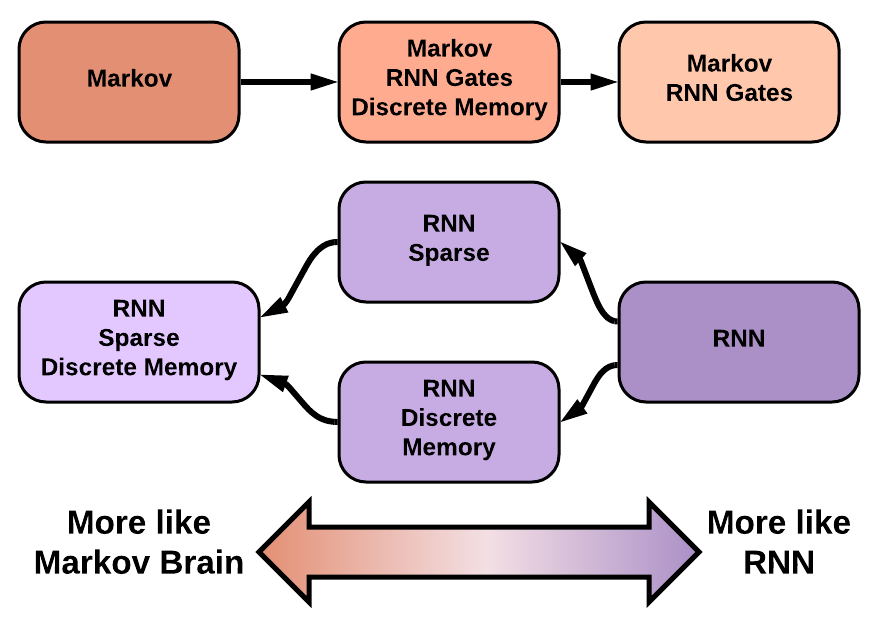
\includegraphics[width=0.4\textwidth]{chapters/2-comp-hybrid/figs/Markov_vs_RNN_H.png}
    \caption{Schematic of hybrids. Orange (top) are Markov-based; purple (bottom) are RNN-based. Arrows indicate a single change away from the canonical brain structure.}
    \label{fig:hybrids}
\end{figure}

\subsubsection{Hybrid Brains}

We implemented a number of features in RNNs and Markov Brains to allow us to create ``hybrid" brains based on each brain type (see Fig~\ref{fig:hybrids}). 
These hybrids are representative of the architectural changes described above which theoretically transform one brain type into the other, and allow us to make those changes in a step-wise fashion, one change at a time.

For Markov brains, we implemented an RNN gate that can stand in place of the canonical lookup table gate. 
These gates have the same node summation and threshold properties as the RNNs. 
The wiring of the RNN gates is sparse and determined by the same genetic encoding as the lookup table gates with the exception that these gates have from 1 to 8 inputs and a single output. 
This replacement constitutes the change to the logical operator described above. 
To approximate the difference in the range of memory values, we added a setting so that memory is either bitted (i.e. mapped to binary such that values of 0 or less are set to 0 and values greater then 0 are set to 1) as in canonical Markov brains, or continuous as in canonical RNNs. 
These changes allow us to test three Markov-based brain variants: a canonical Markov Brain, a Markov-RNN hybrid with discrete memory (i.e. RNN gate with bitted memory), and a Markov-RNN hybrid with continuous memory (i.e. RNN gate without bitted memory). 

In RNN brains, we directly varied the sparsity of their wiring and the discretization of memory. 
To implement sparsity, we biased the genome conversion so that wires with weight 0 were as common as wires with non-zero values. 
This meant that the inital population of randomly generated sparse brains would have on average half as many active connections as fully connected brains. 
As this ratio was only established at initialization, and not enforced thereafter, it could change as a result of evolution. 
To implement the discretization of memory, we added a bitting setting as in the Markov Brains. 
We tested four RNN variants: a canonical RNN, a sparse RNN (i.e. biased weights), a discretized RNN (i.e. bitted memory), and a sparse and discretized RNN (i.e. both biased weights and bitted memory).

\subsection{Worlds}

\begin{figure*}
    \centering
    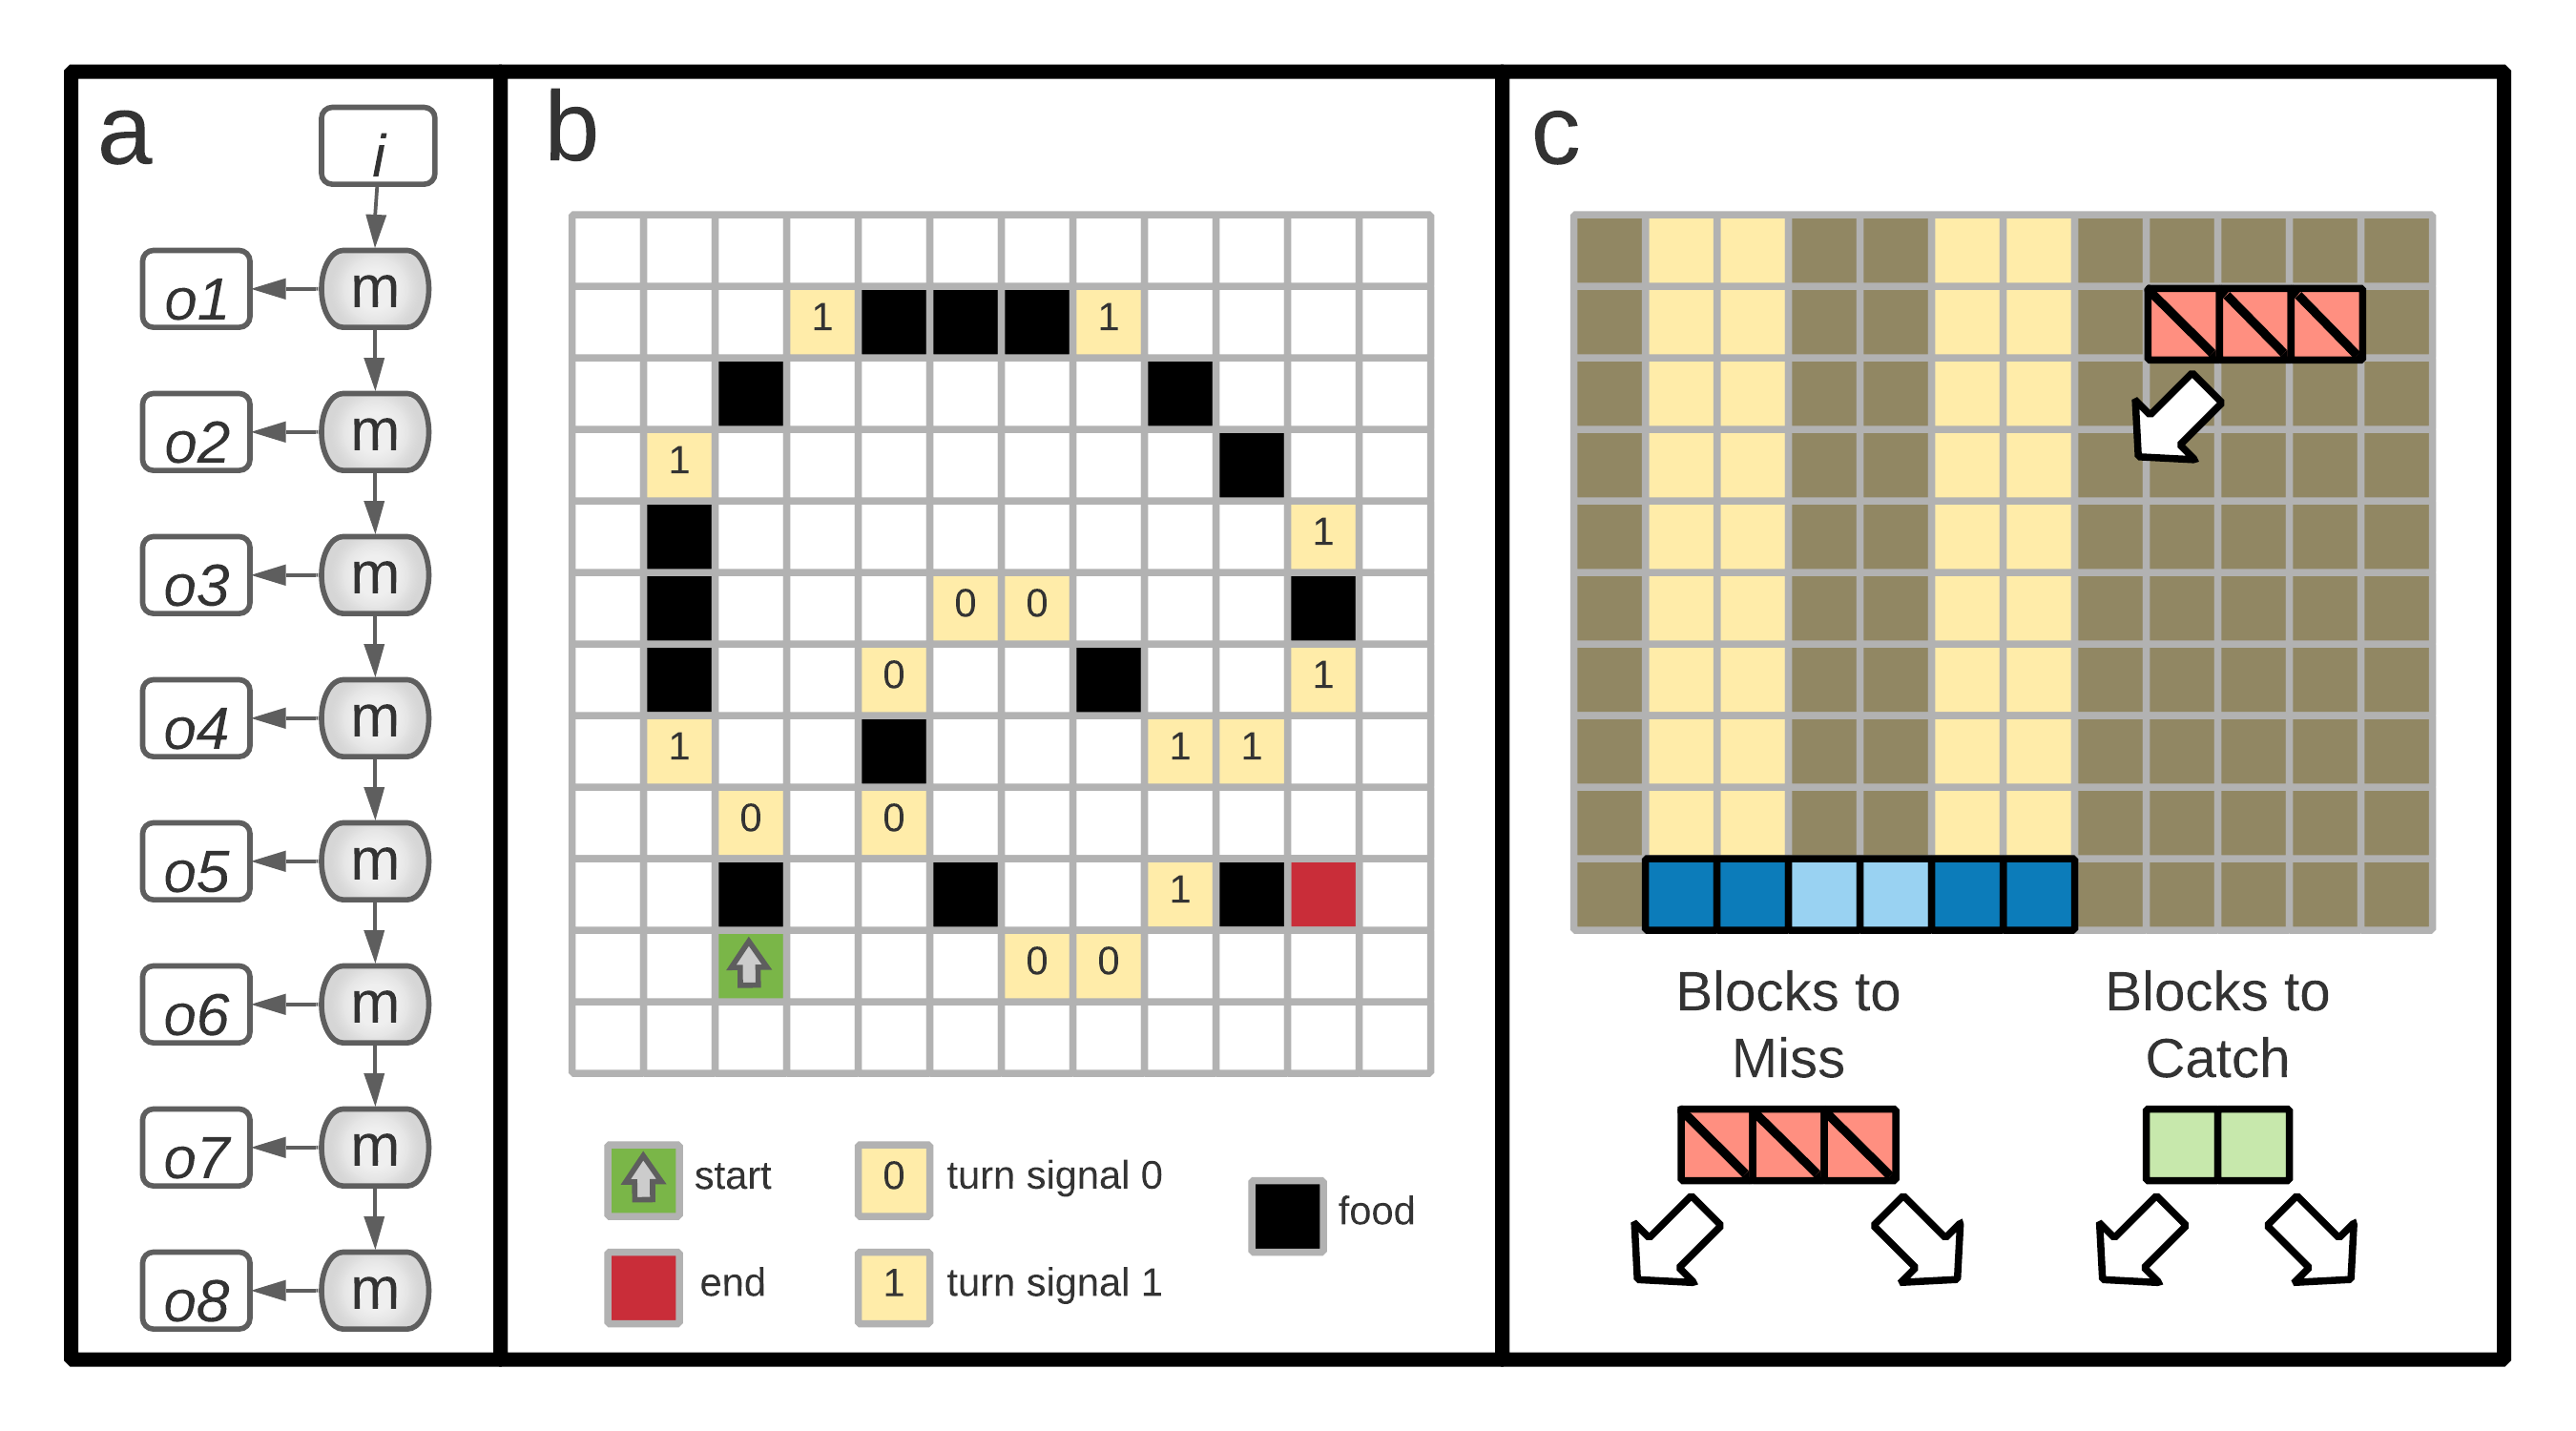
\includegraphics[width=4.5in]{chapters/2-comp-hybrid/figs/ALIFE_2021_SI_Worlds.png}
    \caption{Depictions of the worlds on which the brains were evolved. (A) \textbf{NBack.} Visualization of the data flow required to perform the NBack 8 task of recalling the previous 8 given bits. Here $i$ represents input, $m$ represents memory, and $o1$ through $o8$ represent outputs. (B) \textbf{PathFollow.} Example map from the PathFollow task. Agents start on the green start square facing in the direction of the path. Black indicates path locations with food, where the agent must move forward and which the agent is rewarded for visiting. Yellow indicates locations with randomized turn signals which the agent must associate with either left of right turn. Red indicates the end of the path. Agents that reach the end of the path receive an additional reward if they have visited all "food" locations. (C) \textbf{BlockCatch.} Spatial layout of the BlockCatch task. Blue indicates the agent; dark blue indicates the location of the sensors. Bright yellow indicates the area visible to the sensors, while darker yellow indicates area that is not visible in the agent's current location. Green (blank) and red (hatched) depict blocks that should be caught or missed and arrows indicate possible lateral motion of blocks as they fall.}
    \label{fig:worlds}
\end{figure*}

Since our work is motivated by understanding learning in the context of computational architectures, we tested each of our hybrid brains on three learning-based tasks with diverse characteristics. 
One task dealt primarily with short term memory (NBack), the second with simple information integration and lifetime memory (PathFollow), and the third with more complex information integration and lifetime memory (BlockCatch). 
We provide an in-depth analysis of the required logic and information integration required for each task and thoughts about how this relates to the results in the Discussion section titled Information Integration.

%To test the brains we evolved each brain type in three worlds (i.e. tasks or environments).

\subsubsection{NBack World}
NBack world (Fig~\ref{fig:worlds}) presents a simple short-term memory task. 
In this task, agents are presented a bit stream, one bit at a time, and must respond with the last 8 bits they were provided. 
We tested each agent 10 times with 18 inputs presented per test. 
Only the outputs associated with the last 10 inputs were evaluated. 
Agents received a score based on the ratio of the correct outputs to the total number of outputs.
NBack is based on a common cognitive task in neuropsychology to test working memory via neuroimaging, though its efficacy in human subjects is under review \citep{owen_n-back_2005, miller_is_2009, jaeggi_concurrent_2010}.

\subsubsection{PathFollow World}
In PathFollow world (Fig~\ref{fig:worlds}B), agents must learn to respond to a variable environmental clue. 
Agents exist on a grid and are able to sense symbols only on the space they are currently occupying. 
Agents must use those symbols to navigate a path defined by food and randomized turn signals. 
Agents can move forward and backwards, and turn left and right 45 degrees. 
Each location in the world contains a symbol that marks that location either as start, end, empty, food, turn signal 0, or turn signal 1. 
Agents start on the start location oriented towards the next step on the path. 
Visting a food location provides reward (used to determine reproductive success) and indicates a continuation of the path. 
If the agent steps off the path they receive a small penalty. 
The two turn signals indicate turns in the path, but these signals' meaning are reset every time an agent starts a new path. 
That is, signal 0 may indicate a left turn or a right turn, and signal 1 will indicate the opposite of the direction of signal 0. 
In order to perform well in Path Follow world, agents must form an association between the turn signals and their meaning by trial and error, and then must remember these associations for the remainder of that path.
Agents are scored on their ability to reach the end of the path while visiting all locations and minimizing time off the path.
PathFollow world is a simplified version of the task presented in \cite{pontes_evolutionary_2020}; in the previous work, the turn signals were not restricted to a binary choice.

\subsubsection{BlockCatch World}
BlockCatch world (Fig~\ref{fig:worlds}C) is a task that requires both lifetime memory and complex information integration. 
Agents are rewarded based on whether they catch or avoid a block that falls towards them \citep{marstaller_evolution_2013}. 
The world is a $20 \times 20$ grid, and agents are paddles that move left and right at the bottom of the world. 
Agents are 6 units wide and have 4 sensors that look up and can detect if there is an object directly above them, but not the distance to the object. 
The sensors are positioned such that the agent has a 2 unit wide blind spot over its center. 
Blocks of either size 2 or 3 begin at the top of the world and fall toward the agent one at a time. 
The blocks fall by moving horizontally one space, either left or right, and vertically down one space at a time. 
If a block is size 2 the agent should "catch" the block (i.e. be positioned such that block intersects some part of the agent when the block has fallen to the level of the agent), and if a block is size 3 the agent should "miss" the block. 
Agents must integrate sensor input over time both to determine the block shape (to decide whether to catch or avoid) and the direction the block is moving (to correctly position themselves). 
They therefore must also remember the block size and direction once they have detected these features and behave accordingly. 
Agents are tested on every combination of block size and direction and receive a score that is the ratio of correct results over all tests.

\subsubsection{Experiment Details}
Each described brain variant was evolved on each described world 100 times (i.e. 100 replicates of each experiment) for 200,000 generations.
In all cases, we used populations of 100 agents and tournament selection (size 5). 
Agents' genomes were vectors of integer values in the range [0,255] with initial length 5,000. On reproduction, offsprings' genomes could be altered by insertion and deletion mutations of size 128 to 512 at a per site rate of 0.00002 and point mutations at a per site rate of 0.005. 
Genomes could not mutate to be shorter then 2,000 sites or longer than 20,000 sites.

Markov Brain genomes were seeded in the first generation of each experiment with six gate ``start codons'' for either lookup table gates or RNN gates depending on the brain variant.

All source code for the project, including analysis and visualization scripts, can be found at \url{https://doi.org/10.5281/zenodo.4765681}.